\documentclass[10pt,twocolumn]{article}
\setlength\textwidth{6.875in}
\setlength\textheight{8.875in}
% set both margins to 2.5 pc
\setlength{\oddsidemargin}{-0.1875in}% 1 - (8.5 - 6.875)/2
\setlength{\evensidemargin}{-0.1875in}
\setlength{\marginparwidth}{0pc}
\setlength{\marginparsep}{0pc}%
\setlength{\topmargin}{0in} \setlength{\headheight}{0pt}
\setlength{\headsep}{0pt}
\setlength{\footskip}{37pt}%
\setlength{\columnsep}{0.3125in}
\setlength{\columnwidth}{3.28125in}% (6.875 - 0.3125)/2 = 3.28125in
\setlength{\parindent}{1pc}
\newcommand{\myMargin}{1.00in}
\usepackage[top=\myMargin, left=\myMargin, right=\myMargin, bottom=\myMargin, nohead]{geometry}
\usepackage{epsfig,graphicx}
\usepackage{palatino}
\usepackage{fancybox}
\usepackage[procnames]{listings}
\usepackage{hyperref}

\newenvironment{commentary}
{ \vspace{-0.1in}
  \begin{quotation}
  \noindent
  \small \em
  \rule{\linewidth}{1pt}\\
}
{
  \end{quotation}
}

\title{Chisel 2.0 Manual}
\author{Jonathan Bachrach, Huy Vo, Krste Asanovi\'{c} \\
EECS Department, UC Berkeley\\
{\tt  \{jrb|huytbvo|krste\}@eecs.berkeley.edu}
}
\date{\today}

\newenvironment{example}{\VerbatimEnvironment\begin{footnotesize}\begin{Verbatim}}{\end{Verbatim}\end{footnotesize}}
\newcommand{\kode}[1]{\begin{footnotesize}{\tt #1}\end{footnotesize}}

\def\code#1{{\small\tt #1}}

\def\note#1{\noindent{\bf [Note: #1]}}
%\def\note#1{}

% "define" Scala
\usepackage[T1]{fontenc}  
\usepackage[scaled=0.82]{beramono}  
\usepackage{microtype} 

\sbox0{\small\ttfamily A}
\edef\mybasewidth{\the\wd0 }

\lstdefinelanguage{scala}{
  morekeywords={abstract,case,catch,class,def,%
    do,else,extends,false,final,finally,%
    for,if,implicit,import,match,mixin,%
    new,null,object,override,package,%
    private,protected,requires,return,sealed,%
    super,this,throw,trait,true,try,%
    type,val,var,while,with,yield},
  sensitive=true,
  morecomment=[l]{//},
  morecomment=[n]{/*}{*/},
  morestring=[b]",
  morestring=[b]',
  morestring=[b]"""
}

\usepackage{color}
\definecolor{dkgreen}{rgb}{0,0.6,0}
\definecolor{gray}{rgb}{0.5,0.5,0.5}
\definecolor{mauve}{rgb}{0.58,0,0.82}

% Default settings for code listings
\lstset{frame=tb,
  language=scala,
  aboveskip=3mm,
  belowskip=3mm,
  showstringspaces=false,
  columns=fixed, % basewidth=\mybasewidth,
  basicstyle={\small\ttfamily},
  numbers=none,
  numberstyle=\footnotesize\color{gray},
  % identifierstyle=\color{red},
  keywordstyle=\color{blue},
  commentstyle=\color{dkgreen},
  stringstyle=\color{mauve},
  frame=single,
  breaklines=true,
  breakatwhitespace=true,
  procnamekeys={def, val, var, class, trait, object, extends},
  procnamestyle=\ttfamily\color{red},
  tabsize=2
}

\lstnewenvironment{scala}
{\lstset{language=scala}}
{}
\lstnewenvironment{cpp}
{\lstset{language=C++}}
{}
\lstnewenvironment{bash}
{\lstset{language=bash}}
{}
\lstnewenvironment{verilog}
{\lstset{language=verilog}}
{}



\lstset{frame=}

\begin{document}
\maketitle{}

% TODO: default
% TODO: enum yields UInt
% TODO: why hardware construction languages



\section{Introduction}

This document is a manual for {\em Chisel} (Constructing Hardware In a
Scala Embedded Language).  Chisel is a hardware construction language
embedded in the high-level programming language Scala.  A separate
Chisel tutorial document provides a gentle introduction to using
Chisel, and should be read first.  This manual provides a
comprehensive overview and specification of the Chisel language, which
is really only a set of special class definitions, predefined objects,
and usage conventions within Scala.  When you write a Chisel program
you are actually writing a Scala program.  In this manual, we presume
that you already understand the basics of Scala.  If you are
unfamiliar with Scala, we recommend you consult one of the excellent
Scala books (\cite{programming-scala}, \cite{programming-in-scala}).

\section{Nodes}

Any hardware design in Chisel is ultimately represented by a graph of
node objects.  User code in Chisel generate this graph of nodes, which
is then passed to the Chisel backends to be translated into Verilog or
C++ code.  Nodes are defined as follows:

\begin{scala}
class Node {
  // name assigned by user or from introspection
  var name: String = ""
  // incoming graph edges
  def inputs: ArrayBuffer[Node]
  // outgoing graph edges
  def consumers: ArrayBuffer[Node]
  // node specific width inference
  def inferWidth: Int
  // get width immediately inferrable
  def getWidth: Int
  // get first raw node
  def getRawNode: Node
  // convert to raw bits 
  def toBits: Bits
  // convert to raw bits 
  def fromBits(x: Bits): this.type
  // return lit value if inferrable else null
  def litOf: Lit
  // return value of lit if litOf is non null
  def litValue
    (default: BigInt = BigInt(-1)): BigInt
}
\end{scala}


The uppermost levels of the node class hierarchy are shown in
Figure~\ref{fig:node-hierarchy}.  The basic categories are:

\begin{description}
\item[Lit] -- constants or literals,
\item[Op] -- logical or arithmetic operations,
\item[Updateable] -- conditionally updated nodes,
\item[Data] -- typed wires or ports,
\item[Reg] -- positive-edge-triggered registers, and
\item[Mem] -- memories.
\end{description}

\begin{figure}[h]
\centering
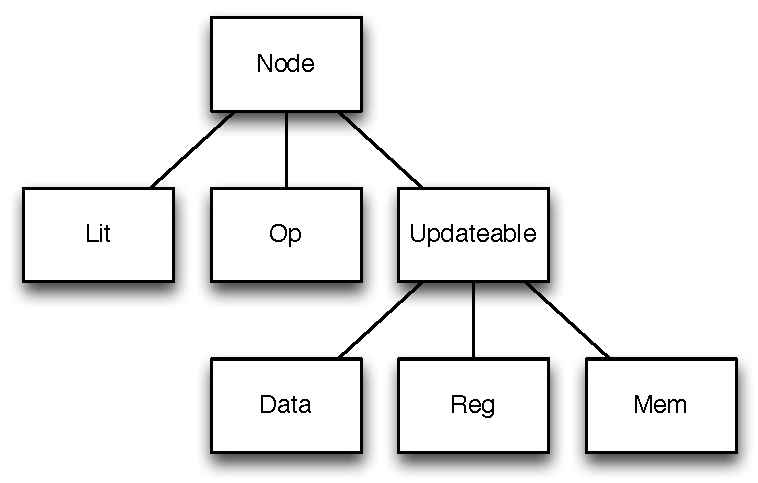
\includegraphics[width=3in]{figs/node-hierarchy.pdf}
\caption{Node hierarchy.}
\label{fig:node-hierarchy}
\end{figure}

\section{Lits}

Raw literals are represented as \code{Lit} nodes defined as follows:

\begin{scala}
class Lit extends Node {
  // original value
  val inputVal: BigInt
}
\end{scala}

\noindent
Raw literals contain a collection of bits.  
Users do not create raw literals directly, but instead use type
constructors defined in Section~\ref{sec:types}.

% Constant or literal values are expressed using Scala integers or strings passed to constructors for the types:

% TODO: isLit and litOf

\section{Ops}

Raw operations are represented as \code{Op} nodes defined as follows:

\begin{scala}
class Op extends Node {
  // op name used during emission
  val op: String
}
\end{scala}

\noindent
Ops compute a combinational function of their inputs.

\section{Types}
\label{sec:types}

A Chisel graph representing a hardware design contains {\em raw} and
{\em type} nodes.  The Chisel type system is maintained separately
from the underlying Scala type system, and so type nodes are
interspersed between raw nodes to allow Chisel to check and respond to
Chisel types.  Chisel type nodes are erased before the hardware design
is translated into C++ or Verilog.  The \code{getRawNode} operator
defined in the base Node class, skips type nodes and returns the first
raw node found.  Figure~\ref{fig:type-hierarchy} shows the built-in
Chisel type hierarchy, with \code{Data} as the topmost node.

\begin{figure}[h]
\centering
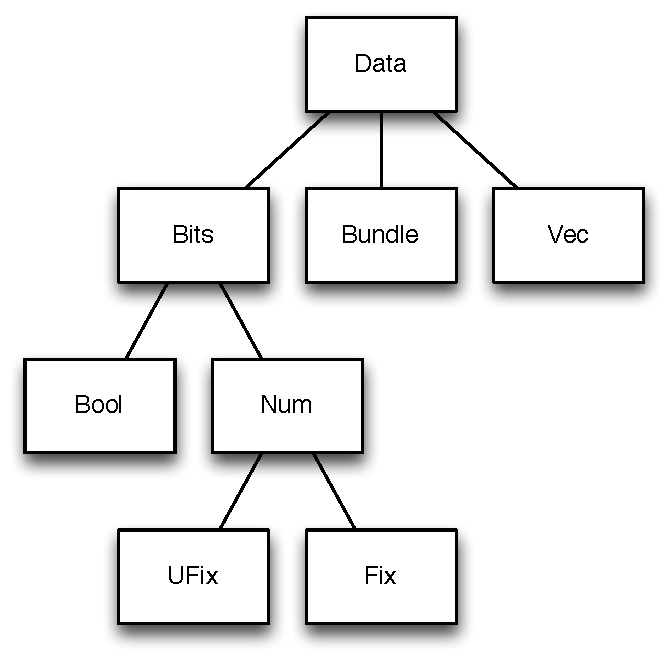
\includegraphics[height=2.5in]{figs/type-hierarchy.pdf}
\caption{Chisel type hierarchy.}
\label{fig:type-hierarchy}
\end{figure}

\noindent
Built-in scalar types include \code{SInt},
\code{UInt}, and \code{Bool}, and built-in aggregate types \code{Bundle} and
\code{Vec} allow the user to expand the set of Chisel datatypes with
collections of other types.

\code{Data} itself is a node:
\begin{scala}
abstract class Data extends Node {
  override def clone(): this.type =
    this.getClass.newInstance.
      asInstanceOf[this.type]
  // simple conversions
  def toSInt: SInt
  def toUInt: UInt
  def toBool: Bool
  def toBits: Bits
  // flatten out to leaves of tree
  def flatten: Array[(String, Data)]
  // port direction if leaf
  def dir: PortDir
  // change dir to OUTPUT
  def asOutput: this.type
  // change dir to INPUT
  def asInput: this.type
  // change polarity of dir
  def flip: this.type
  // assign to input
  def :=[T <: Data](t: T)
  // bulk assign to input
  def <>(t: Data)
}
\end{scala}
\noindent
The Data class has methods for converting between types and for
delegating port methods to its single input.  We will discuss ports in
Section~\ref{sec:ports}.  Finally, users can override the \code{clone}
method in their own type nodes (e.g., bundles) in order to reflect
construction parameters that are necessary for cloning.

Data nodes can be used for four purposes:

\begin{itemize}
\item {\bf types} -- \kode{UInt(width = 8)} -- record intermediate types in the graph
  specifying at minimum bitwidth (described in this section), 
\item {\bf wires} -- \kode{UInt(width = 8)} -- serve as forward declarations of data allowing future
  conditional updates (described in Section~\ref{sec:wires}), 
\item {\bf ports} -- \kode{UInt(dir = OUTPUT, width = 8)} -- are
  specialized wires defining module interfaces, and
  additionally specify direction (described in
  Section~\ref{sec:ports}), and
\item{\bf literals} -- \kode{UInt(1)} or \kode{UInt(1, 8)} -- can be constructed using type object
constructors specifying their value and optional width.
\end{itemize}

\subsection{Bits}

In Chisel, a raw collection of bits is represented by the \code{Bits}
type defined as follows:

\begin{scala}
object Bits {
  def apply(dir: PortDir = null,
            width: Int = -1): Bits
  // create literal from BigInt or Int
  def apply(value: BigInt, width: Int = -1): Bits
  // create literal from String using 
  // base_char digit+ string format
  def apply(value: String, width: Int = -1): Bits
}

abstract class Bits extends Data {
  // bitwise-not
  def unary_~(): Bits
  // bitwise-and
  def &  (b: Bits): Bits
  // bitwise-or
  def |  (b: Bits): Bits
  // bitwise-xor
  def ^  (b: Bits): Bits
  // and-reduction
  def andR(): Bool
  // or-reduction
  def orR():  Bool
  // xor-reduction
  def xorR():  Bool
  // logical NOT
  def unary_!(): Bool
  // logical AND
  def && (b: Bool): Bool
  // logical OR
  def || (b: Bool): Bool
  // equality
  def ===(b: Bits): Bool
  // inequality
  def != (b: Bits): Bool
  // logical left shift
  def << (b: UInt): Bits
  // logical right shift
  def >> (b: UInt): Bits
  // concatenate
  def ## (b: Bits): Bits
  // extract single bit, LSB is 0
  def apply(x: Int): Bits
  // extract bit field from end to start bit pos
  def apply(hi: Int, lo: Int): Bits
}

def Cat[T <: Data](elt: T, elts: T*): Bits
\end{scala}

\noindent
Bits has methods for simple bit operations.  
Note that \code{\#\#} is binary
concatenation, while \code{Cat} is an n-ary concatentation.
To avoid colliding with Scala's builtin \code{==},
Chisel's bitwise comparison is named \code{===}.

A field of width \code{n} can be created from a single bit using \code{Fill}:
\begin{scala}
def Fill(n: Int, field: Bits): Bits
\end{scala}

\noindent
and two inputs can be selected using \code{Mux}:

\begin{scala}
def Mux[T <: Data](sel: Bits, cons: T, alt: T): T
\end{scala}

\noindent

Constant or literal values are expressed using Scala integers or
strings passed to constructors for the types:
\begin{scala}
UInt(1)       // decimal 1-bit lit from Scala Int.
UInt("ha")    // hex 4-bit lit from string.
UInt("o12")   // octal 4-bit lit from string.
UInt("b1010") // binary 4-bit lit from string.
\end{scala}

\noindent
producing a \code{Lit} as shown in the
leftmost subfigure of Figure~\ref{fig:bits-expressions}.

Operations return an actual operator node with a type node combining
the input type nodes.  See Figure~\ref{fig:bits-expressions} for
successively more complicated examples.

\begin{figure*}
\begin{center}
\begin{tabular}{ccc}
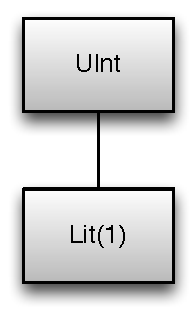
\includegraphics[height=0.94in]{figs/bits-1.pdf} &
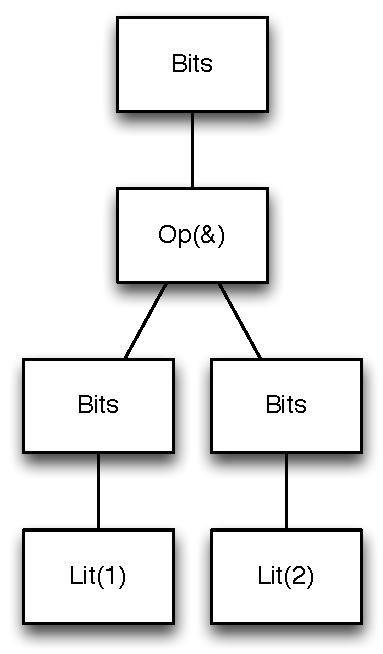
\includegraphics[height=1.96in]{figs/bits-and.pdf} &
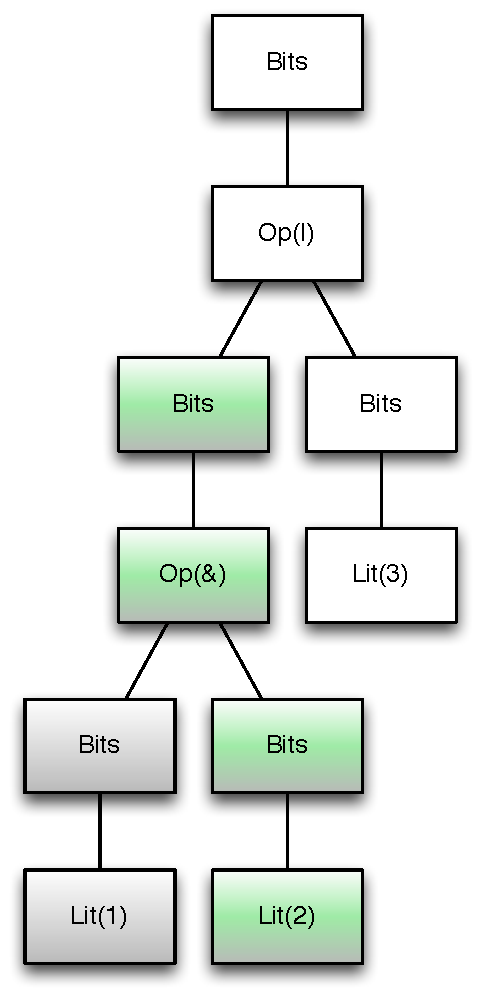
\includegraphics[height=3.0in]{figs/bits-or-and.pdf} \\
\kode{a = UInt(1)} & \kode{b = a \& UInt(2)} &
\kode{b | UInt(3)} \\
\end{tabular}
\end{center}
\caption{Chisel Op/Lit graphs constructed with algebraic expressions
  showing the insertion of type nodes.}
\label{fig:bits-expressions}
\end{figure*}


\subsection{Nums}

\code{Num} is a type node which defines arithmetic operations:

\begin{scala}
class Num extends Bits {
  // Negation
  def unary_-(): Bits
  // Addition
  def +(b: Num): Num
  // Subtraction
  def -(b: Num): Num
  // Multiplication
  def *(b: Num): Num
  // Greater than
  def >(b: Num): Bool
  // Less than
  def <(b: Num): Bool
  // Less than or equal
  def <=(b: Num): Bool
  // Greater than or equal
  def >=(b: Num): Bool
}
\end{scala}

%  // Modulus
%  def %(b: Num): Num
%  // Division
%  def /(b: Num): Num

Signed and unsigned integers
are considered subsets of fixed-point numbers and are represented by
types \code{SInt} and \code{UInt} respectively:

\begin{scala}
object SInt {
  def apply (dir: PortDir = null, 
             width: Int = -1): SInt
  // create literal
  def apply (value: BigInt, width: Int = -1): SInt
  def apply (value: String, width: Int = -1): SInt
}

class SInt extends Num 

object UInt {
  def apply(dir: PortDir = null,
            width: Int = -1): UInt
  // create literal
  def apply(value: BigInt, width: Int = -1): UInt
  def apply(value: String, width: Int = -1): UInt
}

class UInt extends Num {
  // arithmetic right shift
  override def >> (b: UInt): SInt
}
\end{scala}

\noindent
Signed fixed-point
numbers, including integers, are represented using two's-complement
format.  

\subsection{Bools}

Boolean values are represented as \code{Bool}s:

\begin{scala}
object Bool {
  def apply(dir: PortDir = null): Bool
  // create literal
  def apply(value: Boolean): Bool
}

class Bool extends UInt
\end{scala}

\noindent
\code{Bool} is equivalent to \code{UInt(width = 1)}.

\subsection{Bundles}

Bundles group together several named fields of potentially different
types into a coherent unit, much like a \code{struct} in C:

\begin{scala}
class Bundle extends Data {
  // shallow named bundle elements
  def elements: ArrayBuffer[(String, Data)]
}
\end{scala}

\noindent
The name and type of each element in a Bundle can be obtained with the
\code{elements} method, and the \code{flatten} method returns the
elements at the leaves for nested aggregates.  Users can define new
bundles by subclassing \code{Bundle} as follows:

\begin{scala}
class MyFloat extends Bundle {
  val sign        = Bool()
  val exponent    = UInt(width = 8)
  val significand = UInt(width = 23)
}
\end{scala}
\noindent
Elements are accessed using Scala field access:

\begin{scala}
val x  = new MyFloat()
val xs = x.sign
\end{scala}

The names given to a bundle's elements when they are emitted by a C++
or Verilog backend are obtained from their bundle field names, using
Scala introspection.

\subsection{Vecs}

Vecs create an indexable vector of elements: 

\begin{scala}
object Vec {
  def apply[T <: Data](elts: Seq[T]): Vec[T]
  def apply[T <: Data](elt0: T, elts: T*): Vec[T]
  def fill[T <: Data](n: Int)(type: => T): Vec[T]
  def tabulate[T <: Data](n: Int)
        (type: (Int) => T): Vec[T]
  def tabulate[T <: Data](n1: Int, n2: Int)
        (type: (Int, Int) => T): Vec[Vec[T]]
}

class Vec[T <: Data](n: Int, val type: () => T) 
    extends Data {
  def apply(idx: UInt): T
  def apply(idx: Int): T
  def forall(p: T => Bool): Bool
  def exists(p: T => Bool): Bool
  def contains[T <: Bits](x: T): Bool
  def count(p: T => Bool): UInt
  def indexWhere(p: T => Bool): UInt
  def lastIndexWhere(p: T => Bool): UInt
}
\end{scala}

\noindent
with \code{n} elements of type defined with the \code{gen} thunk.
Users can access elements statically with an \code{Int} index or
dynamically using a \code{UInt} index, 
where dynamic access creates a virtual type node (representing a read
``port'') that records the read using the given address.  In either case,
users can wire to the result of a read as follows:

\begin{scala}
v(a) := d
\end{scala}

Read-only memories can be expressed as Vecs of literals:

\begin{scala}
val rom = Vec(UInt(3), UInt(7), UInt(4), UInt(0)) { UInt(width=3) }
val dout = rom(addr)
\end{scala}

% TODO: conditionally assigning to elements

\subsection{Bit Width Inference}

Users are required to set bit widths of ports and registers, but otherwise,
bit widths on nodes are automatically inferred unless set manually by
the user (using \code{Extract} or \code{Cat}).
The bit-width inference engine starts from the graph's input ports and 
calculates node output bit widths from their respective input bit widths according to the following set of rules:\\[-2mm]

{\small
\begin{tabular}{ll}
{\bf operation} & {\bf bit width} \\ 
\verb|z = x + y| & \verb+wz = max(wx, wy)+ \\
\verb+z = x - y+ & \verb+wz = max(wx, wy)+\\
\verb+z = x & y+ & \verb+wz = min(wx, wy)+ \\
\verb+z = Mux(c, x, y)+ & \verb+wz = max(wx, wy)+ \\
\verb+z = w * y+ & \verb!wz = wx + wy! \\
\verb+z = x << n+ & \verb!wz = wx + maxNum(n)! \\
\verb+z = x >> n+ & \verb+wz = wx - minNum(n)+ \\
\verb+z = Cat(x, y)+ & \verb!wz = wx + wy! \\
\verb+z = Fill(n, x)+ & \verb+wz = wx * maxNum(n)+ \\
% \verb+z = x < y+ & \verb+<= > >= && || != ===+ & \verb+wz = 1+ \\
\end{tabular}
}
\\[1mm]
\noindent  
where for instance $wz$ is the bit width of wire $z$, and the \verb+&+
rule applies to all bitwise logical operations.

The bit-width inference process continues until no bit width changes.
Except for right shifts by known constant amounts, the bit-width
inference rules specify output bit widths that are never smaller than
the input bit widths, and thus, output bit widths either grow or stay
the same.  Furthermore, the width of a register must be specified by
the user either explicitly or from the bitwidth of the reset value.
From these two requirements, we can show that the bit-width inference
process will converge to a fixpoint.

\section{Updateables}

\label{sec:wires}

When describing the operation of wire and state nodes, it is often
useful to give the specification as a series of conditional updates to
the output value and to spread out these updates across several
separate statements.  For example, the output of a Data node can be
referenced immediately, but its input can be set later.
\code{Updateable} represents a conditionally updateable node, which
accumulates accesses to the node and which can later generate muxes to
combine these accesses in the circuit.

\begin{scala}
abstract class Updateable extends Node {
  // conditional reads
  def reads: Queue[(Bool, UInt)]
  // conditional writes
  def writes: Queue[(Bool, UInt, Node)]
  // gen mux integrating all conditional writes
  def genMuxes(default: Node)
  override def := (x: Node): this.type
}
\end{scala}

Chisel provides conditional update rules in the form of the
\code{when} construct to support this style of sequential logic
description:
 
\begin{scala}
object when {
  def apply(cond: Bool)(block: => Unit): when
}

class when (prevCond: Bool) {
  def elsewhen (cond: Bool)(block: => Unit): when
  def otherwise (block: => Unit): Unit
}
\end{scala}

\noindent
\code{when} manipulates a global condition stack with dynamic scope.
Therefore, \code{when} creates a new condition that is in force across
function calls.  For example:

\begin{scala}
def updateWhen (c: Bool, d: Data) =
  when (c) { r := d }
when (a) { 
  updateWhen(b, x)
}
\end{scala}

\noindent
is the same as:

\begin{scala}
when (a) { 
  when (b) { r := x } 
}
\end{scala}

% TODO: talk about conds

Chisel provides some syntactic sugar for other common forms of
conditional updates:

\begin{scala}
def unless(c: Bool)(block: => Unit) = 
  when (!c) { block )
\end{scala}

\noindent 
and

\begin{scala}
def otherwise(block: => Unit) = 
  when (Bool(true)) { block }
\end{scala}

We introduce the \code{switch} statement for conditional updates
involving a series of comparisons against a common key:

\begin{scala}
def switch(c: UInt)(block: => Unit): Unit

def is(v: Bool)(block: => Unit)
\end{scala}

\section{Forward Declarations}

Purely combinational circuits are not allowed to have cycles between
nodes, and Chisel will report an error if such a cycle is detected.
Because they do not have cycles, legal combinational circuits can
always be constructed in a feed-forward manner, by adding new nodes
whose inputs are derived from nodes that have already been defined.
Sequential circuits naturally have feedback between nodes, and so it
is sometimes necessary to reference an output wire before the
producing node has been defined.  Because Scala evaluates program
statements sequentially, we have allowed data nodes to serve as a wire
providing a declaration of a node that can be used immediately, but
whose input will be set later.  For example, in a simple CPU, we need
to define the \verb!pcPlus4!  and \verb!brTarget! wires so they can be
referenced before definition:
\begin{scala}
val pcPlus4  = UInt()
val brTarget = UInt()
val pcNext   = Mux(pcSel, brTarget, pcPlus4)
val pcReg    = Reg(data = pcNext)
pcPlus4     := pcReg + UInt(4)
...
brTarget    := addOut
\end{scala}

\noindent
The wiring operator
\verb!:=! is used to wire up
the connection after \verb!pcReg! and \verb!addOut! are defined.
After all assignments are made and the circuit is being elaborated, 
it is an error if a forward declaration is unassigned.

\section{Regs}

The simplest form of state element supported by Chisel is a
positive-edge-triggered register defined as follows:

\begin{scala}
object Reg {
  def apply[T <: Data]
    (type: T = null, 
     data: T = null, 
     init: T = null): T
}

class Reg extends Updateable
\end{scala}

\noindent
where it can be constructed as follows:

\begin{scala}
val r1 = Reg(data = io.in)
val r2 = Reg(init = UInt(1, 8))
val r3 = Reg(data = io.in, reset = UInt(1))
val r4 = Reg(UInt(width = 8))
\end{scala}

\noindent
where \code{init} is the value a reg takes on when implicit
\code{reset} is \code{Bool(true)}.

\section{Mems}

Chisel supports random-access memories via the Mem construct.  Writes to Mems
are positive-edge-triggered and reads are either combinational or
positive-edge-triggered.  

\begin{scala}
object Mem {
  def apply[T <: Data](type: T, depth: Int, 
          seqRead: Boolean = false): Mem
}

class Mem[T <: Data](type: T, depth: Int,
      seqRead: Boolean = false)
    extends Updateable {
  def apply(idx: UInt): T
}
\end{scala}

Ports into Mems are created by applying a \code{UInt} index.  A 32-entry
register file with one write port and two combinational read ports might be
expressed as follows:

\begin{scala}
val rf = Mem(UInt(width = 64), 32)
when (wen) { rf(waddr) := wdata }
val dout1 = rf(waddr1)
val dout2 = rf(waddr2)
\end{scala}

If the optional parameter seqRead is set, Chisel will attempt to infer
sequential read ports when the read address is a Reg.  A one-read,
one-write SRAM might be described as follows:

\begin{scala}
val ram1r1w =
  Mem(UInt(width = 32), 1024, seqRead = true)
val reg_raddr = Reg(UInt())
when (wen) { ram1r1w(waddr) := wdata }
when (ren) { reg_raddr := raddr }
val rdata = ram1r1w(reg_raddr)
\end{scala}

Single-ported SRAMs can be inferred when the read and write conditions are
mutually exclusive in the same \code{when} chain:

\begin{scala}
val ram1p = 
  Mem(UInt(width = 32), 1024, seqRead = true)
val reg_raddr = Reg(UInt())
when (wen) { ram1p(waddr) := wdata }
.elsewhen (ren) { reg_raddr := raddr }
val rdata = ram1p(reg_raddr)
\end{scala}

If the same Mem address is both written and sequentially read on the same clock
edge, or if a sequential read enable is cleared, then the read data is
undefined.

Mem also supports write masks for subword writes.  A given bit is written if
the corresponding mask bit is set.

\begin{scala}
val ram = Mem(UInt(width = 32), 256)
when (wen) { ram.write(waddr, wdata, wmask) }
\end{scala}

\section{Ports}
\label{sec:ports}

Ports are \code{Data} derived nodes used as interfaces to hardware
modules.   A port is a directional version of a primitive
\code{Data} object.  Port directions are defined as follows:

\begin{scala}
trait PortDir
object INPUT  extends PortDir
object OUTPUT extends PortDir
\end{scala}

\noindent
Aggregate ports can be recursively constructed using either a vec or
bundle with instances of \code{Port}s as leaves.  

\section{Modules}

In Chisel, {\em modules} are very similar to {\em modules} in
Verilog, defining a hierarchical structure in the generated circuit.
The hierarchical module namespace is accessible in downstream tools
to aid in debugging and physical layout.  A user-defined module is
defined as a {\em class} which:
\begin{itemize}
\item inherits from \code{Module},
\item contains an interface Bundle stored in a field named \code{io}, and
\item wires together subcircuits in its constructor.
\end{itemize}

Users write their own modules by subclassing Module which is
defined as follows:

\begin{scala}
abstract class Module {
  val io: Bundle
  var name: String = ""
  def compileV: Unit
  def compileC: Unit
}
\end{scala}

\noindent
and defining their own \code{io} field.  For example, to define a two
input mux, we would define a module as follows:

\begin{scala}
class Mux2 extends Module {
  val io = new Bundle{
    val sel = Bool(INPUT)
    val in0 = Bool(INPUT)
    val in1 = Bool(INPUT)
    val out = Bool(OUTPUT)
  }
  io.out := (io.sel & io.in1) | (~io.sel & io.in0)
}
\end{scala}

\noindent
The \code{:=} assignment operator, used in the body of a
module definition, is a special operator in Chisel that wires the input of
left-hand side to the output of the right-hand side.  It is typically
used to connect an output port to its definition.

The \code{<>} operator bulk connects interfaces of opposite gender between
sibling modules or interfaces of same gender between parent/child modules. 
Bulk connections connect leaf ports using pathname matching.
Connections are only made if one of the ports is non-null,
allowing users to repeatedly bulk-connect partially filled interfaces.
After all connections are made and the circuit is being elaborated,
Chisel warns users if ports have other than exactly one connection to them.

The names given to the nodes and submodules stored in a module
when they are emitted by a C++ or Verilog backend are obtained from
their module field names, using Scala introspection.

% TODO: what is same name -- is it a pathname?

\section{BlackBox}

Black boxes allow users to define interfaces to circuits defined
outside of Chisel.  The user defines:

\begin{itemize}
\item a module as a subclass of \code{BlackBox} and
\item an \code{io} field with the interface.
\end{itemize}

\noindent
For example, one could define a simple ROM blackbox as:

\begin{scala}
class RomIo extends Bundle {
  val isVal = Bool(INPUT)
  val raddr = UInt(INPUT,  32)
  val rdata = UInt(OUTPUT, 32)
}

class Rom extends BlackBox {
  val io = new RomIo()
}
\end{scala}

\section{Printf and Sprintf}

Chisel provides the ability to format and print strings for debugging
purposes.  The \code{printf} and \code{sprintf} construct are similar to their
C namesakes: they take a format string and a variable number of arguments,
then print or return a string, respectively.  During simulation, \code{printf}
prints the formatted string to the console on rising clock edges.
\code{sprintf}, on the other hand, returns the formatted string as a bit
vector.

Supported format specifiers are \code{\%b} (binary number), \code{\%d}
(decimal number), \code{\%x} (hexadecimal number), and \code{\%s} (string
consisting of a sequence of 8-bit extended ASCII characters).  (\code{\%\%}
specifies a literal \code{\%}.) Unlike in C, there are no width modifiers: the
bit width of the corresponding argument determines the width in the string
representation.

The following example prints the line \code{"0x4142 16706 AB"} on cycles when
\code{c} is true:

\begin{scala}
val x = Bits(0x4142)
val s1 = sprintf("%x %s", x, x);
when (c) { printf("%d %s\n", x, s1); }
\end{scala}

\section{Assert}

Runtime assertions are provided by the \code{assert} construct.  During
simulation, if an assertion's argument is false on a rising clock edge,
an error is printed and simulation terminates.  For example, the following
will terminate simulation after ten clock cycles:

\begin{scala}
val x = Reg(init = UInt(0, 4))
x := x + UInt(1)
assert(x < UInt(10))
\end{scala}

\section{Main and Testing}

In order to construct a circuit, 
the user calls \code{chiselMain} from their top level \code{main} function:

\begin{scala}
object chiselMain {
  def apply[T <: Module]
    (args: Array[String], comp: () => T): T
}
\end{scala}

\noindent
which when run creates C++ files named
\code{{\it module\_name}.cpp} and \code{{\it module\_name}.h} in
the directory specified with
\code{--targetDir {\it dir\_name}} argument.

% \begin{scala}
% class TestIO
%   (val format: String, val args: Seq[Data] = null)
% 
% class Scanner extends TestIO
% 
% class Printer extends TestIO
% 
% object chiselMainDebug {
%   def apply[T <: Module]
%     (args: Array[String], comp: () => T)(
%      scanner: T => TestIO, 
%      printer: T => TestIO)
% }
% \end{scala}
% 
% \noindent
% 
% We can use the \code{chiselMainDebug} call and \code{TestIO} objects as follows:
% 
% \begin{scala}
% object tutorial {
%   def main(args: Array[String]) = {
%     val dargs = args ++ Array("--genHarness")
%     chiselMainDebug(dargs, () => new Mux2())(
%       c => Scanner("%x %x %x",
%                    c.io.sel, c.io.in0, c.io.in1),
%       c => Printer("%x %x %x %x", 
%                    c.io.sel, c.io.in0, c.io.in1, 
%                    c.io.out))
%   }
% }
% \end{scala}
% 
% \noindent
% where the first three hex numbers from each line are read in from
% standard input and bound to the \code{sel}, \code{in0},  and
% \code{in1} inputs of the multiplexer circuit, and the multiplexer
% inputs and \code{out} are printed out in hex format.  
% 
% Alternatively, a user can specify the scanned inputs and printed
% outputs using aggregate data and one format directive per aggregate.  
% For example, the following accomplishes the same scanning / printing
% as above:
% 
% \begin{scala}
% object tutorial {
%   def main(args: Array[String]) = {
%     val dargs = args ++ Array("--genHarness")
%     chiselMainDebug(dargs, () => new Mux2())(
%       c => Scanner("%x", c.io),
%       c => Printer("%x", c.io)
%   }
% }
% \end{scala}
%  
% Using \code{--generate-harness} for \code{Mux2}
% creates a \code{Mux2-emulator.cpp}  and \code{Mux2-makefile} in directory
% specified by \code{--targetDir}.  The user can then compile it using:
% 
% \begin{scala}
% make -f Mux2-makefile
% \end{scala}
% 
% \noindent
% 
% A user can test the multiplexer by creating a test file called
% \code{test.out} containing:
% \begin{scala}
% 0 0 0 0
% 0 0 1 0
% 0 1 0 1
% 0 1 1 1
% 1 0 0 0
% 1 0 1 1
% 1 1 0 0
% 1 1 1 1
% \end{scala}
% 
% \noindent
% and can be compared using a script as follows
% 
% \begin{scala}
% cut -f 1,2,3 -d " " < test | Mux2 > test.out
% diff test.out test
% \end{scala}
 
\begin{figure}
\begin{center}
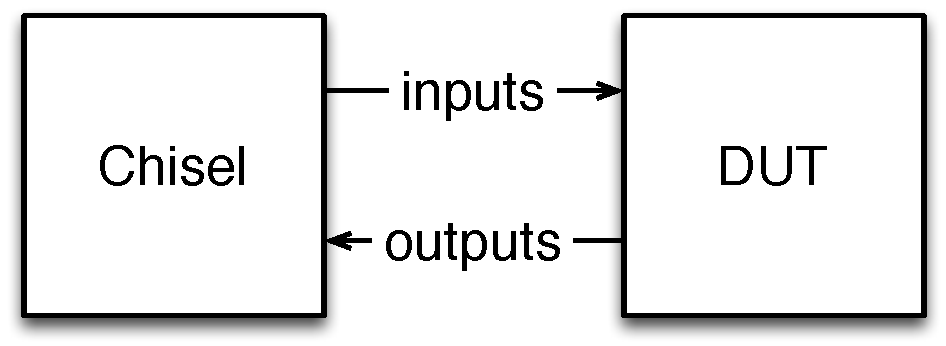
\includegraphics[width=0.45\textwidth]{../tutorial/figs/DUT.pdf}
\end{center}
\caption{DUT run using a Tester object in Scala with stdin and stdout connected}
\label{fig:dut}
\end{figure}
 
Testing is a crucial part of circuit design, 
and thus in Chisel we provide a mechanism for
testing circuits by providing test vectors within Scala using
subclasses of the \code{Tester} class:

\begin{scala}
class Tester[T <: Module]
  (val c: T, val testNodes: Array[Node])
\end{scala}

\noindent
which binds a tester to a module, and specifies the nodes to test,
and finally allows users to write a \code{defTests} function.
The definition for \code{defTests} is:

\begin{scala}
def defTests(body: => Boolean)
\end{scala}

\noindent
where \code{testNodes} are the graph nodes that will be input to and
output from the DUT, and where
users write calls to \code{step} in the body.  Users connect tester
instances to modules using:

\begin{scala}
object chiselMainTest {
  def apply[T <: Module]
    (args: Array[String], comp: () => T)(
     tester: T => Tester[T]): T
}
\end{scala}

\noindent
When \code{--test} is given as an argument to \code{chiselMain}, a
tester instance runs the Design Under Test (DUT) in a separate
process with stdin and stdout connected so that inputs can be sent to
the DUT and outputs can received from the DUT as shown in
Figure~\ref{fig:dut}.
\noindent

\begin{scala}
def step(vars: HashMap[Node, Node]): Boolean
\end{scala}

\noindent
where \code{vars} is a mapping of test nodes to literals, 
with assignments to input nodes being sent to the DUT and assignments to
non-input nodes being interpreted as expected values.
\code{test} first sends inputs specifed in vars, steps the DUT and then either
compares expected values from vars or sets vars for test nodes without
entries in \code{vars}.
The following is an example for defining tests for \code{Mux2}:

\begin{scala}
class Mux2Tests(c: Mux2) 
    extends Tester(c, Array(c.io)) {  
  defTests {
    var allGood = true
    val n = pow(2, 3).toInt
    val vars = new HashMap[Node, Node]()
    for (s <- 0 until 2) {
    for (i0 <- 0 until 2) {
    for (i1 <- 0 until 2) {
      vars(c.io.sel) = UInt(s)
      vars(c.io.in1) = UInt(i1)
      vars(c.io.in0) = UInt(i0)
      vars(c.io.out) = UInt(if (s == 1) i1 else i0)
      allGood &&= step(vars)
    } } } 
    allGood
  }
}
\end{scala}

\noindent
and the following shows how it is invoked:

\begin{scala}
chiselMainTest(args + "--test", () => new Mux2()){ 
  c => new Mux2Tests(c) 
}
\end{scala}

% The app exits with its return code equal to all test vectors not matching.
% For example, we can test \code{Mux2} using the following:
% 
% \begin{scala}
% object tutorial {
%   val tsts = 
%      Array(Array(0, 0, 0, 0),
%            Array(0, 0, 1, 0),
%            Array(0, 1, 0, 1),
%            Array(0, 1, 1, 1),
%            Array(1, 0, 0, 0),
%            Array(1, 0, 1, 1),
%            Array(1, 1, 0, 0),
%            Array(1, 1, 1, 1))
%   def main(args: Array[String]) = {
%     val targs = args ++ Array("--genHarness") 
%     chiselMainTest(targs, () => new Mux2())(
%       c => Printer("%x", c.io),
%       c => Tester(tsts, c.io)
%    )
%   }
% }
% \end{scala}

Finally, command arguments for \code{chiselMain*} are as follows: \\

\begin{tabular}{lll}
\verb+--targetDir+ & target pathname prefix \\
\verb+--genHarness+ & generate harness file for C++ \\
\verb+--debug+ & put all wires in C++ class file \\
\verb+--compile+ & compiles generated C++ \\
\verb+--test+ & runs tests using C++ app \\
\verb+--backend v+ & generate verilog \\ 
\verb+--backend c+ & generate C++ (default)\\
\verb+--vcd+ & enable vcd dumping \\
\end{tabular}


\section{C++ Emulator}

The C++ emulator is based on a fast multiword library using
C++ templates.  
A single word is defined by \code{val\_t} as follows: 

\begin{cpp}
typedef uint64_t val_t;
typedef int64_t sval_t; 
typedef uint32_t half_val_t;
\end{cpp}

\noindent
and multiwords are defined by \code{dat\_t} as follows:

\begin{cpp}
template <int w>
class dat_t {
 public:
  const static int n_words;
  inline int width ( void );
  inline int n_words_of ( void );
  inline bool to_bool ( void );
  inline val_t lo_word ( void );
  inline unsigned long to_ulong ( void );
  std::string to_str ();
  static dat_t<w> rand();
  dat_t<w> ();
template <int sw> 
  dat_t<w> (const dat_t<sw>& src);
  dat_t<w> (const dat_t<w>& src);
  dat_t<w> (val_t val);
template <int sw> 
  dat_t<w> mask(dat_t<sw> fill, int n);
template <int dw> 
  dat_t<dw> mask(int n);
template <int n> 
  dat_t<n> mask(void);
  dat_t<w> operator + ( dat_t<w> o );
  dat_t<w> operator - ( dat_t<w> o );
  dat_t<w> operator - ( );
  dat_t<w+w> operator * ( dat_t<w> o );
  dat_t<w+w> fix_times_fix( dat_t<w> o );
  dat_t<w+w> ufix_times_fix( dat_t<w> o );
  dat_t<w+w> fix_times_ufix( dat_t<w> o );
  dat_t<1> operator < ( dat_t<w> o );
  dat_t<1> operator > ( dat_t<w> o );
  dat_t<1> operator >= ( dat_t<w> o );
  dat_t<1> operator <= ( dat_t<w> o );
  dat_t<1> gt ( dat_t<w> o );
  dat_t<1> gte ( dat_t<w> o );
  dat_t<1> lt ( dat_t<w> o );
  dat_t<1> lte ( dat_t<w> o );
  dat_t<w> operator ^ ( dat_t<w> o );
  dat_t<w> operator & ( dat_t<w> o );
  dat_t<w> operator | ( dat_t<w> o );
  dat_t<w> operator ~ ( void );
  dat_t<1> operator ! ( void );
  dat_t<1> operator && ( dat_t<1> o );
  dat_t<1> operator || ( dat_t<1> o );
  dat_t<1> operator == ( dat_t<w> o );
  dat_t<1> operator == ( datz_t<w> o );
  dat_t<1> operator != ( dat_t<w> o );
  dat_t<w> operator << ( int amount );
  dat_t<w> operator << ( dat_t<w> o );
  dat_t<w> operator >> ( int amount );
  dat_t<w> operator >> ( dat_t<w> o );
  dat_t<w> rsha ( dat_t<w> o);
  dat_t<w>& operator = ( dat_t<w> o );
  dat_t<w> fill_bit(val_t bit);
  dat_t<w> fill_byte
    (val_t byte, int nb, int n);
template <int dw, int n> 
  dat_t<dw> fill( void );
template <int dw, int nw> 
  dat_t<dw> fill( dat_t<nw> n );
template <int dw> 
  dat_t<dw> extract();
template <int dw> 
  dat_t<dw> extract(val_t e, val_t s);
template <int dw, int iwe, int iws> 
  dat_t<dw> extract
    (dat_t<iwe> e, dat_t<iws> s);
template <int sw> 
  dat_t<w> inject
    (dat_t<sw> src, val_t e, val_t s);
template <int sw, int iwe, int iws> 
  dat_t<w> inject
    (dat_t<sw> src, 
     dat_t<iwe> e, dat_t<iws> s);
template <int dw> 
  dat_t<dw> log2();
  dat_t<1> bit(val_t b);
  val_t msb();
template <int iw>
  dat_t<1> bit(dat_t<iw> b)
}
\end{cpp}

\begin{cpp}
template <int w, int sw> 
  dat_t<w> DAT(dat_t<sw> dat);
template <int w> 
  dat_t<w> LIT(val_t value);
template <int w> dat_t<w> 
  mux ( dat_t<1> t, dat_t<w> c, dat_t<w> a )
\end{cpp}

\noindent
where \code{w} is the bit width parameter.

The Chisel compiler compiles top level modules into a single flattened \code{mod\_t}
class that can be created and executed:

\begin{cpp}
class mod_t {
 public:
  // initialize module
  virtual void init (void) { };
  // compute all combinational logic
  virtual void clock_lo (dat_t<1> reset) { };
  // commit state updates
  virtual void clock_hi (dat_t<1> reset) { };
  // print printer specd node values to stdout
  virtual void print (FILE* f) { };
  // scan scanner specd node values from stdin
  virtual bool scan (FILE* f) { return true; };
  // dump vcd file
  virtual void dump (FILE* f, int t) { };
};
\end{cpp}

Either the Chisel compiler can create a harness or the user can write
a harness themselves.  The following is an example of a harness for a
CPU module:

\begin{cpp}
#include "cpu.h"

int main (int argc, char* argv[]) {
  cpu_t* c = new cpu_t();
  int lim = (argc > 1) ? atoi(argv[1]) : -1;
  c->init();
  for (int t = 0; lim < 0 || t < lim; t++) {
    dat_t<1> reset = LIT<1>(t == 0);
    if (!c->scan(stdin)) break;
    c->clock_lo(reset);
    c->clock_hi(reset);
    c->print(stdout);
  }
}
\end{cpp}

\section{Verilog}

Chisel generates Verilog when the \code{--v} argument is passed into
\code{chiselMain}.  For example, from SBT, the following

\begin{scala}
run --v
\end{scala}

\noindent
would produce a single Verilog file named \code{{\it module-name}.v} in
the target directory.
The file will contain one module per module defined as submodules of
the top level module created in \code{chiselMain}.  Modules with
the same interface and body are cached and reused.

\section{Multiple Clock Domains}

Chisel 2.0 introduces support of multiple clock domains.  

\subsection{Creating Clock domains}

In order to use multiple clock domains, users must create multiple clocks.  
In Chisel, clocks are first class nodes created with a reset signal parameter and defined as follows:

\begin{scala}
class Clock (reset: Bool) extends Node {
  def reset: Bool // returns reset pin
}
\end{scala}

\noindent
% Having reset in clock makes it easier to pass around.
In Chisel there is a builtin implicit clock that state elements use by default:

\begin{scala}
var implicitClock = new Clock( implicitReset )
\end{scala}

The clock for state elements and modules can be defined using an additional named parameter called clock:

\begin{scala}
Reg(... clock: Clock = implicitClock)
Mem(... clock: Clock = implicitClock)
Module(... clock: Clock = implicitClock)
\end{scala}

\subsection{Crossing Clock Domains}

There are two ways that circuits can be defined to send data between clock domains.
The first and most primitive way is by using a synchronizer circuit comprised of two registers as follows:

\begin{scala}
// signalA is in clock domain clockA, 
// want a version in clockB as signalB
val s1 = Reg(init = UInt(0), clock = clockB)
val s2 = Reg(init = UInt(0), clock = clockB)
s1      := signalA
s2      := s1; 
signalB := s2
\end{scala}

\noindent
Due to metastability issues, this technique is limited to communicating one bit data between domains.

The second and more general way to send data between domains is by using an asynchronous queue:

\begin{scala}
class AsyncQueue[T<:Data](gen: T, depth: Int, enq_clk: Clock, deq_clock: Clock)
  extends Module
\end{scala}

\noindent
We can then get a version of signalA from clock domains clockA to clockB by specifying the standard queue parameters and the two clocks and then using the standard decoupled ready/valid signals:

\begin{scala}
val queue = new AsyncQueue(Uint(width = 32), 2, clockA, clockB)
fifo.enq.bits := signalA
signalB       := fifo.deq.bits
fifo.valid    := condA
fifo.ready    := condB
...
\end{scala}

\subsection{Backend Specific Multiple Clock Domains}

Each Chisel backend requires the user to setup up and control multiple clocks in a backend specific manner.  For the purposes of showing how to drive a multi clock design, consider the example of hardware with two modules communicating using an AsyncQueue with each module on separate clocks: \verb+fastClock+ and \verb+slowClock+.  

\subsubsection{C++}

In the C++ backend, for every clock \verb+i+ there is a
\begin{itemize}
\item \verb+uint64_t clk_i+ field representing the clock \verb+i+'s period,
\item \verb+uint63_t clk_i_cnt+ field representing the clock \verb+i+'s current count,
\item \verb+clock_lo_i+ and \verb+clock_hi_i+, 
\item \verb+int reset()+ function which ensures that all \verb+clock_lo+ and \verb+clock_hi+ functions are called at least once, and
\item \verb+int clock(reset)+ function which computes min delta, invokes appropriate \verb+clock_lo+ and \verb+clock_hi+'s and returns min delta used.
\end{itemize}

\noindent
In order to set up a C++ simulation, the user 
\begin{itemize}
\item initializes all period fields to desired period
\item initializes all count fields to desired phase, 
\item calls \verb+reset+ and then
\item repeated calls clock to step the simulation.
\end{itemize}

\noindent
The following is a C++ example of a main function for the \verb+slowClock+ / \verb+fastClock+ example:

\begin{scala}
int main(int argc, char** argv) {
  ClkDomainTest_t dut;
  dut.init(1);
  dut.clk = 2;
  dut.clk_cnt = 1;
  dut.fastClock = 4;
  dut.fastClock_cnt = 0;
  dut.slowClock = 6;
  dut.slowClock_cnt = 0;
  for (int i = 0; i < 12; i ++) 
    dut.reset();
  for (int i = 0; i < 96; i ++) 
    dut.clock(LIT<1>(0));
}
\end{scala}

\subsubsection{Verilog}

In Verilog, 

\begin{itemize}
\item Chisel creates a new port for each clock / reset,
\item Chisel wires all the clocks to the top module, and
\item the user must create an \verb+always+ block clock driver for every clock \verb+i+.
\end{itemize}

\noindent
The following is a Verilog example of a top level harness to drive the  \verb+slowClock+ / \verb+fastClock+ example circuit:

\begin{scala}
module emulator;
  reg fastClock = 0, slowClock = 0, 
      resetFast = 1, resetSlow = 1;
  wire [31:0] add, mul, test;
  always #2 fastClock = ~fastClock;
  always #4 slowClock = ~slowClock;
  initial begin
     #8 
     resetFast = 0;
     resetSlow = 0;
     #400
     $finish;
  end
  ClkDomainTest dut (
     .fastClock(fastClock),
     .slowClock(slowClock),
     .io_resetFast(resetFast),
     .io_resetSlow(resetSlow),
     .io_add(add), .io_mul(mul), .io_test(test));
endmodule
\end{scala}

\noindent
See \url{http://www.asic-world.com/verilog/verifaq2.html} for more information about simulating clocks in Verilog.

\section{Extra Stuff}

\lstset{language=scala}

\begin{scala}
def ListLookup[T <: Bits]
  (addr: UInt, default: List[T], 
   mapping: Array[(UInt, List[T])]): List[T]

def Lookup[T <: Data]
  (addr: UInt, default: T, 
   mapping: Seq[(UInt, T)]): T

// n-way multiplexor
def MuxCase[T <: Data] 
  (default: T, mapping: Seq[(Bool, T)]): T

// n-way indexed multiplexer:
def MuxLookup[S <: UInt, T <: Data] 
  (key: S, default: T, mapping: Seq[(S, T)]): T
\end{scala}

% TODO: PROBE
% \begin{scala}
% Probe
% \end{scala}

\begin{scala}
// create n enum values of given type
def Enum[T <: UInt](n: Int, type: T): List[T]

// create enum values of given type and names
def Enum[T <: UInt]
  (l: Symbol *)(type: => T): Map[Symbol, T]

// create enum values of given type and names
def Enum[T <: UInt]
  (l: List[Symbol], type: => T): Map[Symbol, T]
\end{scala}

% \section{Name Mangling}
% 
% \begin{itemize}
% \item separate and escape sequence
% \item module prefix
% \item vec element suffixes
% \item naming from fields
% \item bundle field paths
% \item target language reserve word avoidance
% \end{itemize}

\section{Standard Library}

\subsection{Math}

\begin{scala}
// Returns the log base 2 of the input 
// Scala Integer rounded up
def log2Up(in: Int): Int

// Returns the log base 2 of the input
// Scala Integer rounded down
def log2Down(in: Int): Int

// Returns true if the input Scala Integer 
// is a power of 2
def isPow2(in: Int): Boolean

// linear feedback shift register
def LFSR16(increment: Bool = Bool(true)): UInt
\end{scala}

\subsection{Sequential}

\begin{scala}
// Returns the n-cycle delayed version 
// of the input signal
def ShiftRegister[T <: Data](in: T, n: Int): T

def Counter(cond: Bool, n: Int) = {
  val c = Reg(init = UInt(0, log2Up(n)))
  val wrap = c === UInt(n-1)
  when (cond) {
    c := Mux(Bool(!isPow2(n)) && wrap, UInt(0), 
             c + UInt(1))
  }
  (c, wrap && cond)
}
\end{scala}

\subsection{UInt}

\begin{scala}
// Returns the number of bits set in the 
// input signal. Causes an exception if 
// the input is wider than 32 bits.
def PopCount(in: UInt): UInt

// Returns the reverse the input signal
def Reverse(in: UInt): UInt

// returns the one hot encoding of
// the input UInt
def UIntToOH(in: UInt, width: Int): UInt

// does the inverse of UIntToOH
def OHToUInt(in: UInt): UInt
def OHToUInt(in: Seq[Bool]): UInt

// Builds a Mux tree out of the input 
// signal vector using a one hot encoded 
// select signal. Returns the output of 
// the Mux tree
def Mux1H[T <: Data]
      (sel: UInt, in: Vec[T]): T
def Mux1H[T <: Data]
      (sel: Vec[Bool], in: Vec[T]): T

// Builds a Mux tree under the
// assumption that multiple
// select signals can be enabled.
// Priority is given to the first 
// select signal. Returns the output 
// of the Mux tree.
def PriorityMux[T <: Data]
      (sel: UInt, in: Seq[T]): T
def PriorityMux[T <: Data]
      (sel: Seq[UInt], in: Seq[T]): T

// Returns the bit position of the
// trailing 1 in the input vector with
// the assumption that multiple bits of
// the input bit vector can be set
def PriorityEncoder(in: UInt): UInt
def PriorityEncoder(in: Seq[Bool]): UInt

// Returns the bit position of the
// trailing 1 in the input vector with
// the assumption that only one bit in 
// the input vector can be set
def PriorityEncoderOH(in: UInt): UInt
def PriorityEncoderOH(in: Seq[Boo]): UInt
\end{scala}

\subsection{DecoupledIO}

\begin{scala}
// Adds a ready-valid handshaking
// protocol to any interface. The 
// standard used is that the
// consumer uses the flipped
// interface.
class DecoupledIO[+T <: Data](type: T) 
    extends Bundle {
  val ready = Bool(INPUT)
  val valid = Bool(OUTPUT)
  val bits  = type.asOutput
}
object Decoupled {
  def apply (type: T) = new DecoupledIo(type)
}

// Adds a valid protocol to any
// interface. The standard used is
// that the consumer uses the
// flipped interface.
class ValidIO[+T <: Data](type: T) 
    extends Bundle {
  val valid = Bool(OUTPUT)
  val bits  = type.asOutput
}

// Hardware module that is used to 
// sequence n producers into 1 consumer. 
// Priority is given to lower
// producer
// Example usage:
//    val arb = new Arbiter(2, UInt())
//    arb.io.in(0) <> producer0.io.out
//    arb.io.in(1) <> producer1.io.out
//    consumer.io.in <> arb.io.out
class Arbiter[T <: Data](n: Int, type: T) 
  extends Module 

// Hardware module that is used to 
// sequence n producers into 1 consumer.
// Producers are chosen in round robin 
// order
// Example usage:
//    val arb = new RRArbiter(2, UInt())
//    arb.io.in(0) <> producer0.io.out
//    arb.io.in(1) <> producer1.io.out
//    consumer.io.in <> arb.io.out
class RRArbiter[T <: Data](n: Int, type: T) 
  extends Module 

// Generic hardware queue. Required
// parameter entries controls the
// depth of the queues. The width of
// the queue is determined from the 
// inputs.
// Example usage:
//    val q = new Queue(UInt(), 16)
//    q.io.enq <> producer.io.out
//    consumer.io.in <> q.io.deq
class Queue[T <: Data]
    (type: T, entries: Int, 
     pipe: Boolean = false,
     flow: Boolean = false
     flushable: Boolean = false)
    extends Module  

// A hardware module that delays data 
// coming down the pipeline by the 
// number of cycles set by the 
// latency parameter. Functionality
// is similar to ShiftRegister but
// this exposes a Pipe interface.
// Example usage:
//    val pipe = new Pipe(UInt())
//    pipe.io.enq <> produce.io.out
//    consumer.io.in <> pipe.io.deq
class Pipe[T <: Data]
    (type: T, latency: Int = 1) extends Module

\end{scala}

% henry

% \section{Acknowlegements}
% 
% Many people have helped out in the design of Chisel, and we thank them
% for their patience, bravery, and belief in a better way.  Many
% Berkeley EECS students in the Isis group gave weekly feedback as the
% design evolved including but not limited to Yunsup Lee, Andrew
% Waterman, Scott Beamer, Chris Celio, etc.  Yunsup Lee gave us feedback
% in response to the first RISC-V implementation, called TrainWreck,
% translated from Verilog to Chisel.  Andrew Waterman and Yunsup Lee
% helped us get our Verilog backend up and running and Chisel TrainWreck
% running on an FPGA.  Brian Richards was the first actual Chisel user,
% first translating (with Huy Vo) John Hauser's FPU Verilog code to
% Chisel, and later implementing generic memory blocks.  Brian gave many
% invaluable comments on the design and brought a vast experience in
% hardware design and design tools.  Chris Batten shared his fast
% multiword C++ template library that inspired our fast emulation
% library.  Huy Vo became our undergraduate research assistant and was
% the first to actually assist in the Chisel implementation.  We
% appreciate all the EECS students who participated in the Chisel
% bootcamp and proposed and worked on hardware design projects all of
% which pushed the Chisel envelope.  We appreciate the work that James
% Martin and Alex Williams did in writing and translating network and
% memory controllers and non-blocking caches.  Finally, Chisel's
% functional programming and bit-width inference ideas were inspired by
% earlier work on a hardware description language called Gel~\cite{gel} designed in
% collaboration with Dany Qumsiyeh and Mark Tobenkin.
% 
% % \note{Who else?}
% 
\begin{thebibliography}{50}
\bibitem{chisel-dac12} Bachrach, J., Vo, H., Richards, B., Lee, Y., Waterman,
  A., Avi\v{z}ienis, Wawrzynek, J., Asanovi\'{c} \textsl{Chisel:
    Constructing Hardware in a Scala Embedded Language}
in DAC '12.
\bibitem{programming-in-scala}Odersky, M., Spoon, L., Venners,
  B. \textsl{Programming in Scala} by Artima.
\bibitem{programming-scala}Payne, A., Wampler, D.
  \textsl{Programming Scala} by O'Reilly books.
% \bibitem{gel} Bachrach, J., Qumsiyeh, D., Tobenkin, M. \textsl{Hardware Scripting in Gel}.
% in Field-Programmable Custom Computing Machines, 2008. FCCM '08. 16th.
\end{thebibliography}
 

\end{document}
